\chapter[Referencial Teórico]{Referencial Teórico}

\section{Engenharia de Requisitos Orientada a Meta}

\subsection{Requisitos Não-Funcionais}

\subsection{NFR Framework}

O NFR Framework é um modelo intencional que ajuda os desenvolvedores  a  lidar com requisitos não-funcionais através de grafos, que podem ser visualizados na forma interativa e incremental, da análise e revisão de um \textit{Softgoal Interdependency Graphs} - SIGs. O framework possui uma estrutura orientada por processo e pode ser utilizado como complemento nas abordagens tradicionais orientada a produto. Dando suporte aos desenvolvedores em seus \textit{softgoals} e os \textit{tradeoffs} (situações onde existem conflitos de escolha). Diante da complexidade de tratar os RNFs enfrentada pelos desenvolvedores em projetos de software a o tratamento dos RNFs	pode ser facilitado através do uso de catálogos de conhecimento para os RNFs \cite{chung2012non}. 


É através do SIGs que é mantido todo o registro das decisões tomada durante todo o processo de desenvolvimento do software e as decisões de design em forma gráfica e consisa, este registro gráfico possibilita aos desenvolvedores acompanhar as decisões sobre os requisitos não funcionais, as alternativas associadas  ao requisito, decisões e as razões pelas quais as decisões foram tomadas. É no SIGs que surge os principais conceitos do NFR Framework. como \textit{softgoals} que são os principais requisitos e são apresentados como uma nuvem na parte superior do grafo, esses \textit{softgoals} podem ser conectados através de links de interdependência com outros \textit{softgoals} \cite{chung2012non}.

O NFR framework é composto por cinco componentes, sendo eles: Sofgoals, Interdependências, Procedimento de avaliação, Métodos e as Correlações \cite{chung2012non}. Esses elementos serão detalhados abaixo, bem como suas representações gráficas. 

\begin{itemize}
	\item \textit{Softgoals}
	
	É a unidade básica utilizada na representação dos RNFs, podendo assumir as naturezas: Subjetiva, pois o RNF pode variar de acordo com o julgamento de cada pessoa; Relativa, pois o RNF pode depender de algum tipo de relação com algum outro RNF. Existem três tipos de \textit{softgoals}: (i) \textit{Softgoals} de RNFs, que representam os requisitos não funcionais para serem satisfeitos; (ii) \textit{Operationalizing softgoals}, basicamente são as técnicas de desenvolvimento que ajudam a satisfazer o requisito não funcional, elas podem aparecer como uma operação, representação de dados, restrição ou atribuição de um agente externo a uma tarefa; (iii) \textit{Claim sofgoals}, é o tipo que ajuda para a tomada de decisões. A representação gráfica dos tipos de \textit{softgoals} pode ser consultada na figura \ref{fig01}.
	
	\begin{figure}[h]
		\centering
		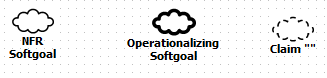
\includegraphics[keepaspectratio=true,scale=0.9]{figuras/tiposDeSoftgoals.png}
		\caption{Representação gráfica dos tipos de \textit{softgoals}.}
		\label{fig01}
	\end{figure} 

	\item Interdependências
	
	É o componente responsável por estabelecer as inter-relações entre os \textit{softgoals}. As interdependências que fazem o registro do refinamento dos \textit{softgoals} em \textit{softgoals} mais específicos (filhos), e suas contribuições para a satisfazer o \textit{softgoal} mais genêrico (pai).  
\end{itemize}

\subsection{i*}

\subsection{FURPS}


\section{Arquitetura de Software}

\subsection{MVC - Model-View-Controller}

\chapter{Metodologia}

\subsection{Classificação da Pesquisa}